\chapter{软件安装}
\section{硬件环境要求说明}
为了满足软件正常运转,硬件环境应满足以下要求:
\begin{itemize}
    \item  内存:512MB以上
    \item  硬盘:20GB以上
    \item  接口:USB或者COM专用接口
    \item  网络:离线
    \item  其他:键盘、鼠标、显示屏
\end{itemize}

\section{软件环境要求说明}
为了满足软件正常运转,软件环境应满足以下要求:
\begin{itemize}
    \item  系统:Window7/Window10
    \item  框架:\textcolor{red}{.NET Framework版本在4.6.1以上}
    \item  驱动:串口驱动程序
\end{itemize}
\subsection{查看系统版本}
\begin{itemize}
    \item 方法1:首先在Windows中搜索\textcolor{red}{'系统信息'},搜到桌面应用\textcolor{red}{'系统信息'},
点击打开,最后进入系统信息中,即可查看到系统的版本号。
    \item 方法2:打开控制面板,点击\textcolor{red}{'管理工具'},即可查看到系统的版本号。
    \item 方法3:在命令提示符界面,输入命令:\textcolor{red}{'Winver'},回车,即可查看到系统的版本号。
\end{itemize}
\subsection{查看目标框架版本}
\par 第一步:在电脑上打开\textcolor{red}{控制面板},点击\textcolor{red}{卸载程序}(见\figref{fig:controlPanel})。
\begin{figure}[H]
    \centering
    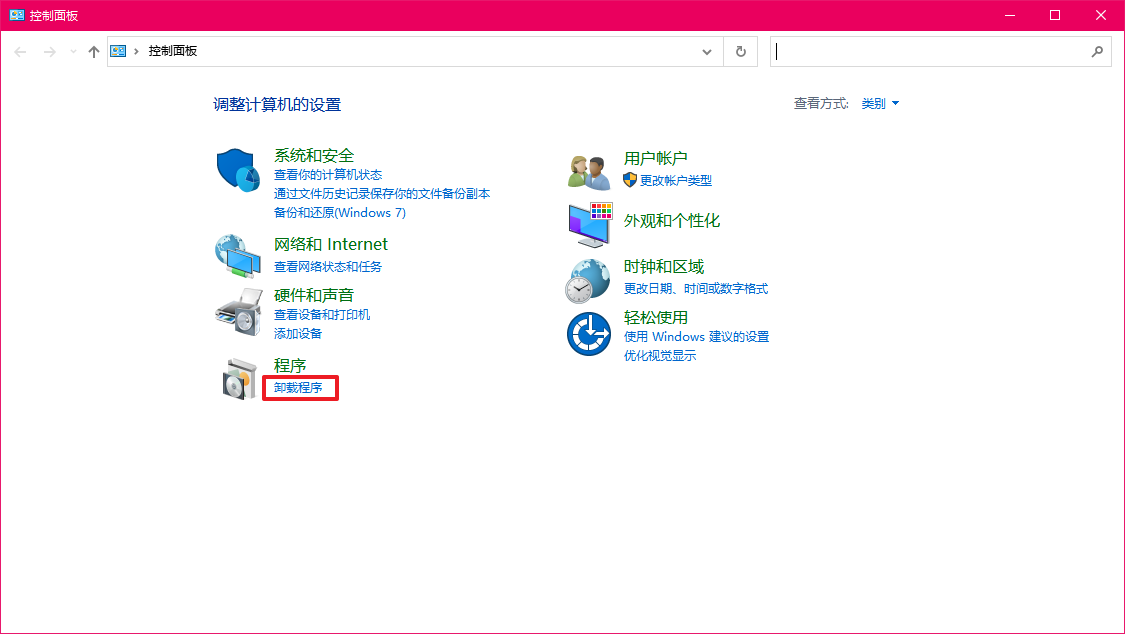
\includegraphics[width=1\textwidth]{installation/controlPanel.png}
    \caption{ 控制面板 \label{fig:controlPanel}}
\end{figure}
\par 第二步:点击打开\textcolor{red}{启用或关闭Windows功能}(见\figref{fig:openWindow})。
\begin{figure}[H]
    \centering
    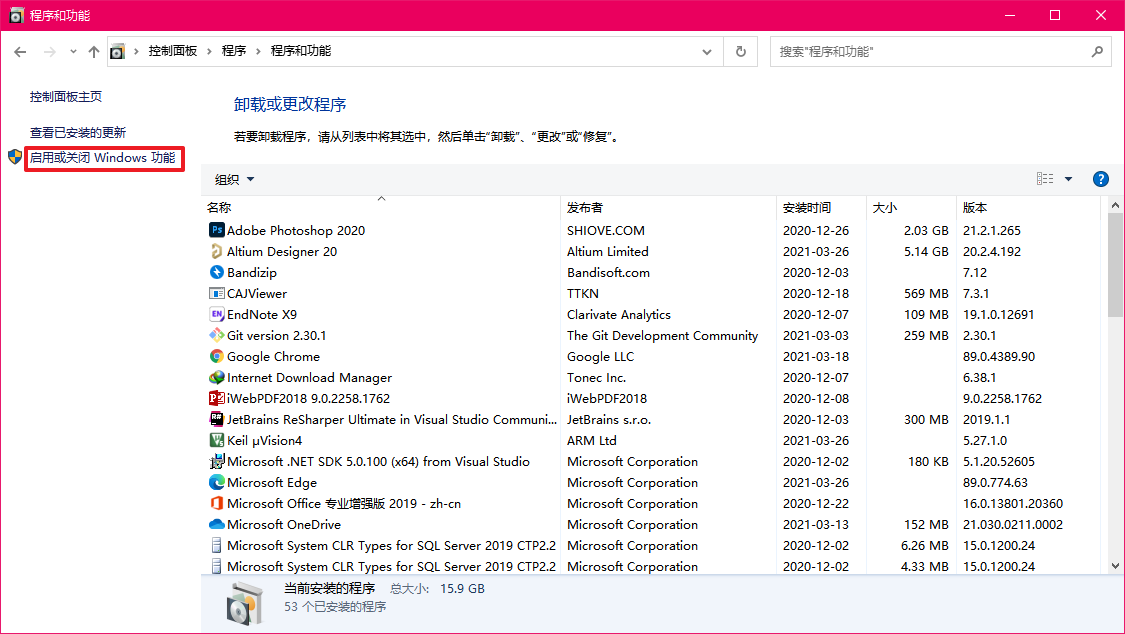
\includegraphics[width=1\textwidth]{installation/openWindow.png}
    \caption{ 启用或关闭Windows功能 \label{fig:openWindow}}
\end{figure}
\par 第三步:进去之后,可以看到.NET Framework版本,有多个版本的话,以高版本为准(见\figref{fig:frameworkVersion})。
\begin{figure}[H]
    \centering
    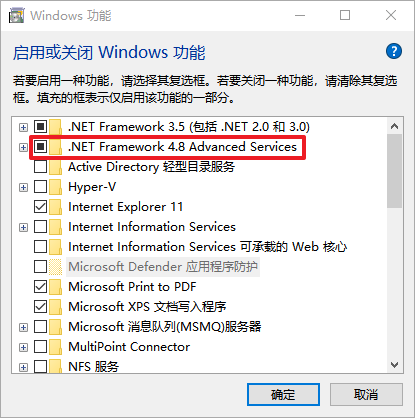
\includegraphics[width=0.6\textwidth]{installation/frameworkVersion.png}
    \caption{ .NET Framework版本 \label{fig:frameworkVersion}}
\end{figure}

\subsection{安装目标框架}
假如目标框架.NET Framework版本在4.6.1以下,进入相应下载地址\textcolor{red}{https://dotnet.micr
osoft.com/download/archives},可选择最新版下载(见\figref{fig:netDownloadArchives}),可选择window系统下的.NET Framework4.8栏目所有版本(见\figref{fig:netDownloads}),
需要下载.NET Framework4.6.1以上版本(见\figref{fig:supportedVersion})。
下载后按照默认设置安装,重启电脑即可。
\begin{figure}[H]
    \centering
    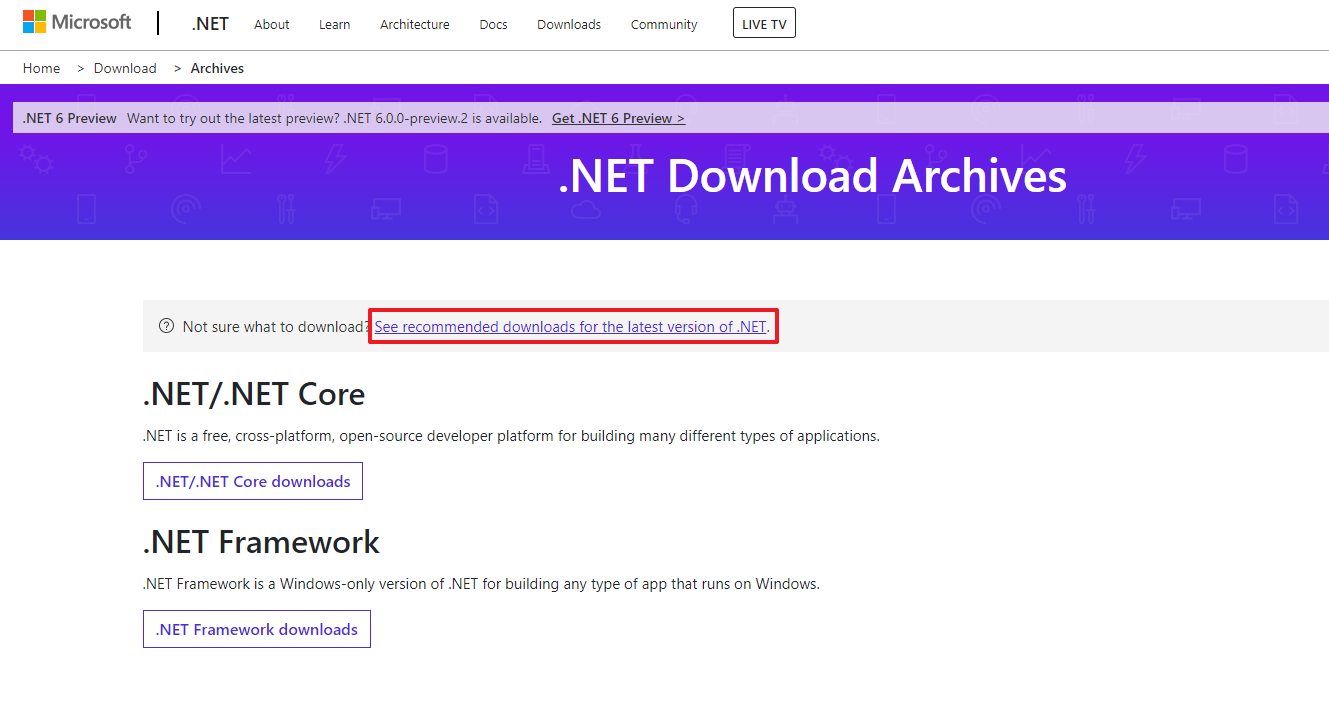
\includegraphics[width=1\textwidth]{installation/netDownloadArchives.png}
    \caption{ .NET Framework下载网站 \label{fig:netDownloadArchives}}
\end{figure}
\begin{figure}[H]
    \centering
    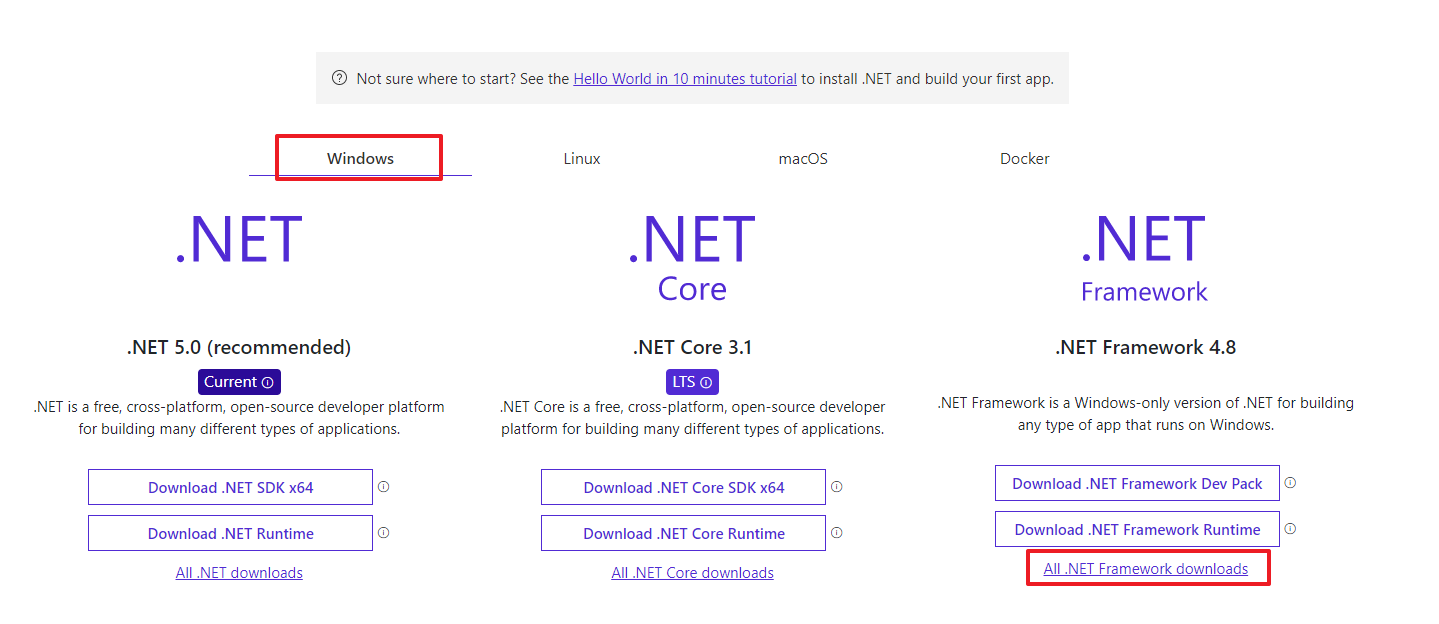
\includegraphics[width=1\textwidth]{installation/netDownloads.png}
    \caption{ .NET Framework选择 \label{fig:netDownloads}}
\end{figure}
\begin{figure}[H]
    \centering
    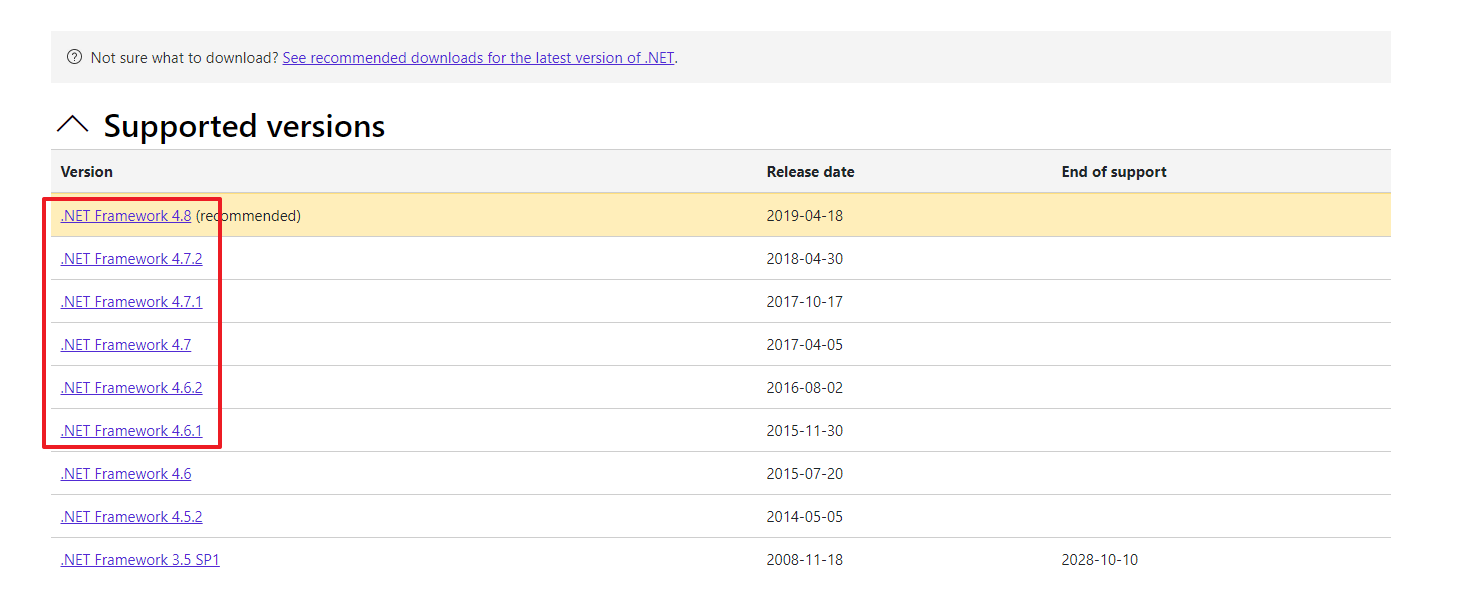
\includegraphics[width=1\textwidth]{installation/supportedVersion.png}
    \caption{ .NET Framework可下载版本 \label{fig:supportedVersion}}
\end{figure}

\section{其它环境要求说明}
\begin{itemize}
    \item 为了满足仪器测量精度,减少环境干扰,整个测试过程应在恒温的封闭实验室进行。
\end{itemize}

\section{建立软件备份}
更新前,需要备份历史测试数据、和系统设置文件。

% 如果条件容许,应该告诉用户如何作系统原介质上软件系统
% 的备份,同时要求用户把系统的原介质作稳妥的保存,用系统的备份介质作系统安装
\section{软件安装过程}
\subsection{安装软件\label{subsec:install}}
\par 本软件为免安装,下载软件包解压即可使用。
\par 第一步:进入下载地址\textcolor{red}{https://github.com/Joe-zhouman/multimeter-public/releases}。
选择对应文件下载到本地(见\figref{fig:downloadPack})。
\begin{figure}[H]
    \centering
    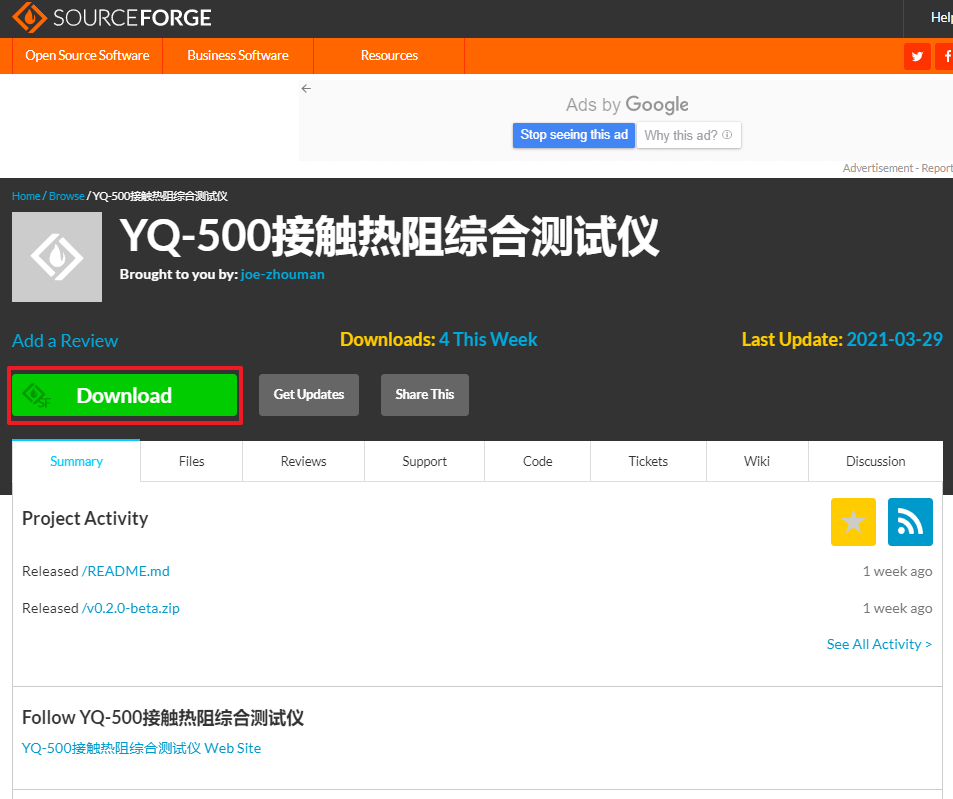
\includegraphics[width=1\textwidth]{installation/downloadPack.png}
    \caption{ 软件下载 \label{fig:downloadPack}}
\end{figure}
\par 第二步:将下载的软件包解压,添加\textcolor{red}{YQ-500接触热阻综合测试仪.exe}快捷方式到电脑桌面,
点击快捷方式即可使用(见\figref{fig:launchFile})。
\begin{figure}[H]
    \centering
    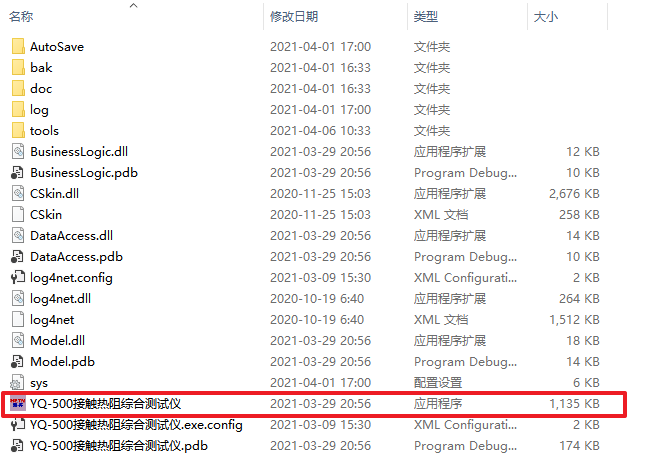
\includegraphics[width=1\textwidth]{installation/launchFile.png}
    \caption{ 启动文件 \label{fig:launchFile}}
\end{figure}
\subsection{安装串口驱动}
\par 由于电脑和数采仪需要串口通信,软件正常使用还需要安装\textcolor{red}{串口驱动程序}。
\par 第一步:打开\nameref{subsec:install}一节下载并解压好的软件包,进入\textcolor{red}{tools}目录(见\figref{fig:toolsFile})。
\begin{figure}[H]
    \centering
    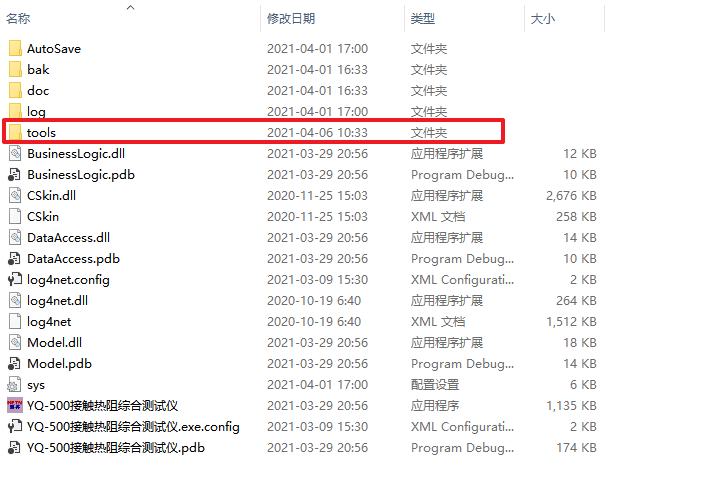
\includegraphics[width=1\textwidth]{installation/toolsFile.png}
    \caption{ 串口驱动文件目录 \label{fig:toolsFile}}
\end{figure}
\par 第二步:解压\textcolor{red}{ZIP 压缩文件 (.zip)}文件,选择对应的系统版本文件(见\figref{fig:toolsVersion})。
\begin{figure}[H]
    \centering
    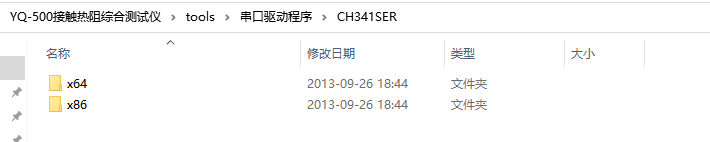
\includegraphics[width=1\textwidth]{installation/toolsVersion.png}
    \caption{ 串口驱动版本选择 \label{fig:toolsVersion}}
\end{figure}
\par 第三步:点击安装文件,右键\textcolor{red}{以管理员身份运行}(见\figref{fig:toolsSetup})。
\begin{figure}[H]
    \centering
    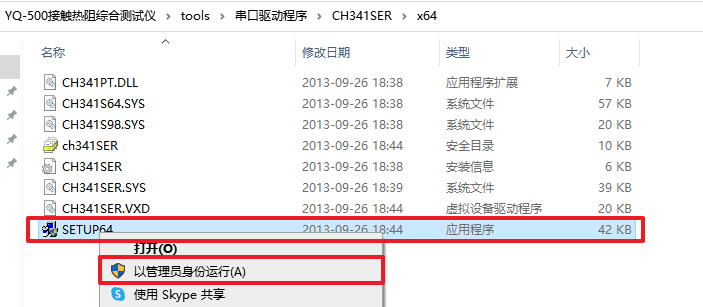
\includegraphics[width=1\textwidth]{installation/toolsSetup.png}
    \caption{ 以管理员身份运行 \label{fig:toolsSetup}}
\end{figure}
\par 第四步:直接点击\textcolor{red}{安装}按钮(见\figref{fig:setupClick})。
\begin{figure}[H]
    \centering
    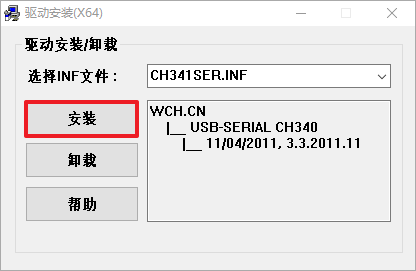
\includegraphics[width=0.6\textwidth]{installation/setupClick.png}
    \caption{ 串口驱动安装 \label{fig:setupClick}}
\end{figure}
\par 第五步:等待,提示\textcolor{red}{驱动预安装成功}后,重启电脑即可(见\figref{fig:setupSucess})。
\begin{figure}[H]
    \centering
    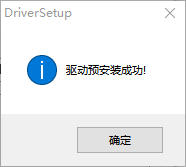
\includegraphics[width=0.4\textwidth]{installation/setupSucess.png}
    \caption{ 串口驱动安装成功 \label{fig:setupSucess}}
\end{figure}
